%%%%%%%%%%%%%%%%%%%%%%%%%%%%%%%%%%%%%%%%%
% Memo
% LaTeX Template
% Version 1.0 (30/12/13)
%
% This template has been downloaded from:
% http://www.LaTeXTemplates.com
%
% Original author:
% Rob Oakes (http://www.oak-tree.us) with modifications by:
% Vel (vel@latextemplates.com)
%
% License:
% CC BY-NC-SA 3.0 (http://creativecommons.org/licenses/by-nc-sa/3.0/)
%
%%%%%%%%%%%%%%%%%%%%%%%%%%%%%%%%%%%%%%%%%

\documentclass[letterpaper,11pt]{texMemo} % Set the paper size (letterpaper, a4paper, etc) and font size (10pt, 11pt or 12pt)

\usepackage{parskip} % Adds spacing between paragraphs
\usepackage[colorlinks]{hyperref}
\usepackage{graphicx}
\usepackage{float}
\usepackage{listings}
\hypersetup{citecolor=DeepPink4}
\hypersetup{linkcolor=red}
\hypersetup{urlcolor=blue}
\usepackage{cleveref}
\setlength{\parindent}{15pt} % Indent paragraphs

%----------------------------------------------------------------------------------------
%	MEMO INFORMATION
%----------------------------------------------------------------------------------------

%----------------------------------------------------------------------------------------
%	MEMO INFORMATION
%----------------------------------------------------------------------------------------

\memoto{Dr.Jeff McGough} % Recipient(s)

\memofrom{Benjamin Lebrun} % Sender(s)

\memosubject{Homework 1} % Memo subject

\memodate{\today} % Date, set to \today for automatically printing todays date

%\logo{\includegraphics[width=0.1\textwidth]{logo.png}} % Institution logo at the top right of the memo, comment out this line for no logo

%----------------------------------------------------------------------------------------

\begin{document}


\maketitle % Print the memo header information

%----------------------------------------------------------------------------------------
%	MEMO CONTENT
%----------------------------------------------------------------------------------------

\section*{Problem 2.10}
\subsection*{Problem statement}
Assume that you have a two link manipulator with $a_1=15$cm and $a_2=15$cm and that the base of the manipulator is at
the origin of the coordinate system. Write a Python program to take the list of workspace points and plug them into the
inverse kinematics formulas for the two link manipulator. Plot these points on a graph where $\theta_1$ is the horizontal
axis and $\theta_2$ is the vertical axis. You will have to adjust some aspects to get a good looking plot.
(Scale factors etc.) Test your code on the workspace line (a) $x+y=25, x,y>0$ and (b) $x=10cos(t)+15, y=10sin(t)$ for $0 \leq t \leq\pi$.
The point here is to see what the configuration space curve looks like.

\subsection*{Solution approach and algorithm description.}
For this problem, we can use the inverse kinematic equations: 
\[
    D = \frac{x^2+y^2-a^2_1-a^2_2}{2a_1 a_2}
\]

\[
    \theta_1 = \tan^{-1}(\frac{y}{x})-\tan^{-1}(\frac{a_2 \sin(\theta_2)}{a_1+a_2 \cos(\theta_2)})
\]

\[
    \theta_2 = \tan^{-1}(\frac{\sqrt(1-D^2)}{D})
\]

And with python code, found the equation for $x+y=25$ in terms of $y$, therefore $y=25-x$ for part A of this question.
These equations are found in section 2.3 of the Roboscience course book, along with some sample code in Python.
We then used the matplotlib library for creating plots to view in a separate opening window. Part B was found by 
simply plotting the $x$ and $y$ coordinates from the equations $x=10cos(t)+15, y=10sin(t)$ via $0 \leq t \leq\pi$ 
and simply using the output of the inverse kinematic equations to plot their results.

\begin{figure}[ht]
\caption{Graphed runs of 10 part A and B}
\centering
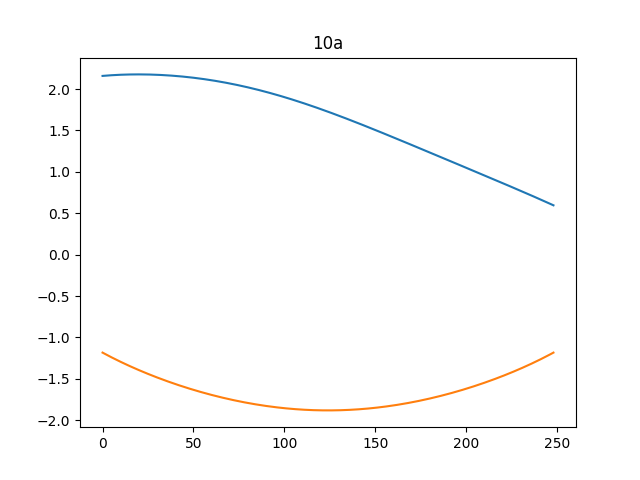
\includegraphics[scale=0.45]{img/10a.png}
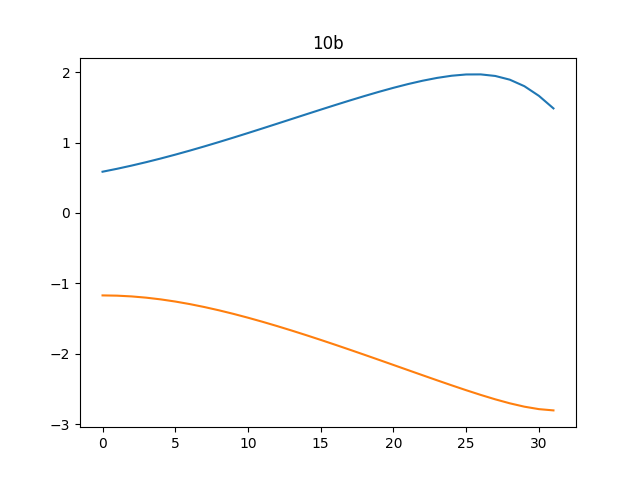
\includegraphics[scale=0.45]{img/10b.png}
\end{figure}

\newpage
\subsection*{Code 10a}
\begin{tiny}
\lstinputlisting{../10a.py}
\end{tiny}

\subsection*{Code 10b}
\begin{tiny}
\lstinputlisting{../10b.py}
\end{tiny}

\newpage
\section*{Problem 2.11}
\subsection*{Problem statement}
Assume that you have a two link manipulator with $a_1=15$cm and $a2=15$cm and that the base of the manipulator
is at the origin of the coordinate system. Write a two link manipulator location program (Python).
This program will take a list of angles and compute the location of the end effector. Show how this
program works with the list of angles you generated in the previous problem. If the angle inputs are
generated by a square, the simulated robot arm’s end effector should trace a square. Plot the end effector
points. You need to plot the input shape and the final shape to see if your code is correct. You will need
to use the previous problem for this problem. Demonstrate your code to trace out the four segments which
form the square with endpoints (5,0), (5, 15), (20, 15), (20,0).

\subsection*{Solution approach and algorithm description.}
For problem 10, we used inverse kinematic equations to find and interpretation from configuration space 
to working space of two systems. If we want to find the inverse of this, we use forward kinematic equations
to find and interpret values in working space to configuration space. Much like inverse kinematics, we have
a collection of equations to find forward kinematic solutions to the two link manipulator problem. 

\[
    x = a_2 \cos(\theta_1+\theta_2) + a_1\cos(\theta_1)
\]

\[
    y = a_2 \sin(\theta_1+\theta_2)+a_1\sin(\theta_1)
\]

Using these expressions in python, we can then derive an interpretation from a set of points to where
they would lie in configuration space. This was done for our linear equation $x+y=25$ and $x=10cos(t)+15, y=10sin(t)$ 
and also a set of points to draw a square.

\begin{figure}[ht]
\caption{Graphed runs of 11 part A, B, and C}
\centering
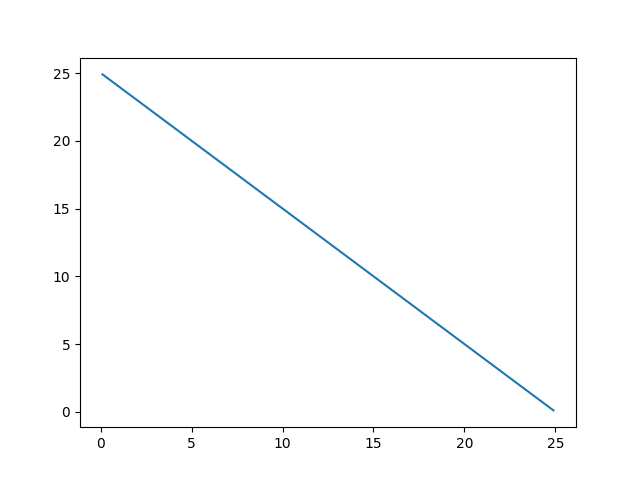
\includegraphics[scale=0.45]{img/11a.png}
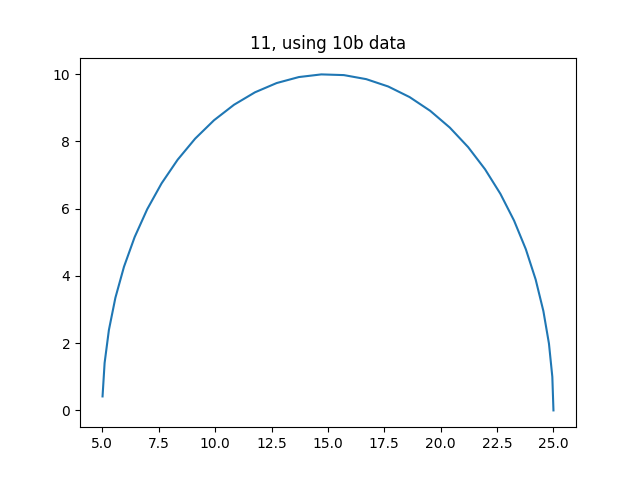
\includegraphics[scale=0.45]{img/11b.png}
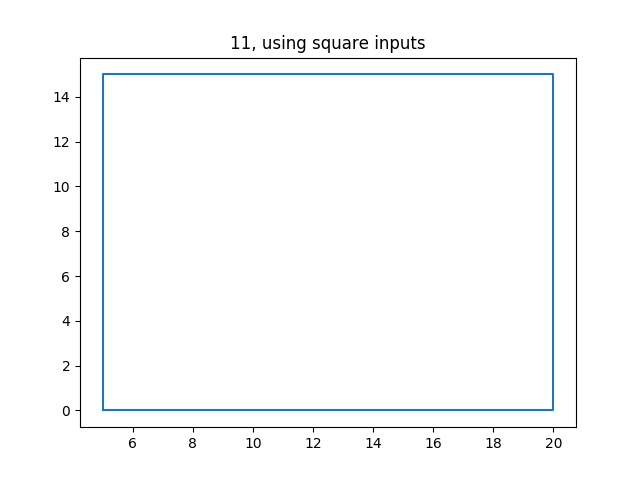
\includegraphics[scale=0.45]{img/11c.png}
\end{figure}

\newpage
\subsection*{Code 11}
\begin{tiny}
\lstinputlisting{../11.py}
\end{tiny}

\newpage
\section*{Problem 2.18}
\subsection*{Problem statement}
Using Numpy and the linspace command, build an array of points for Fig. 2.37. The top is given by $(x-10)^2+(y-8)^2=25$
and the bottom is the line segment along $y=8$. Traverse the figure starting at the right corner, going counter clockwise
(circle first) and ending on the line segment. Check this with the Python plot command. Show the result.

\begin{figure}[h]
\centering
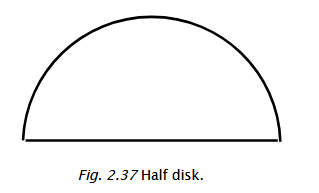
\includegraphics{img/fig237.png}
\end{figure}

\subsection*{Solution approach and algorithm description.}
Numpy linspace attempts to create as linear an array as possible over a set of points. This then allows us to simply define 
an equation where python will interpret the inputs/outputs of this equation as a vector of these points which can then be used
to plot this desired figure. This was done first by solving for $y$ in our given equation, then using inputs of $x$ across the
range $5 \leq x < 15 $ where the half circle and the segment of $y=8$ meet.

\subsection*{Code 18}
\begin{tiny}
\lstinputlisting{../18.py}
\end{tiny}

\begin{figure}[ht]
\caption{Graphed run of 18}
\centering
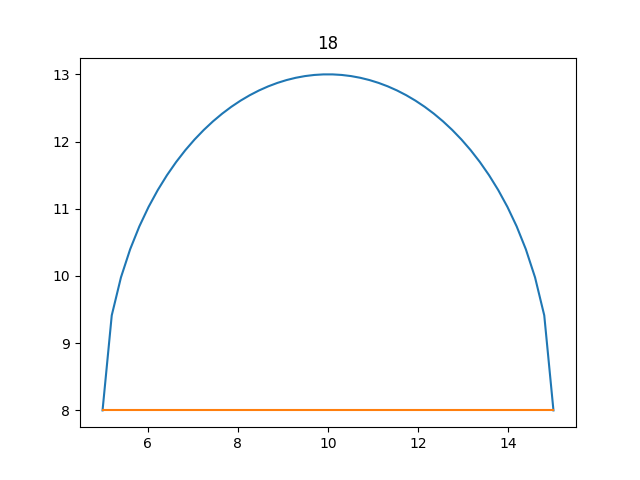
\includegraphics[scale=0.7]{img/18.png}
\end{figure}

\newpage
\section*{Problem 2.29}
\subsection*{Problem statement}
Given a differential drive robot starting from (0,0,0) find the final position when wheel
velocities are given by:

$t=0$ to $t=5$: $\omega_1=2$, $\omega_2=2$

$t=5$ to $t=6$: $\omega_1=3$, $\omega_2=4$

$t=6$ to $t=10$: $\omega_1=1$, $\omega_2=2$

where $D=10$, $L=16$.

\subsection*{Solution approach and algorithm description.}


\end{document}